\chapter{Charakterisierung und Vorbereitung des Datensatzes}
Der verwendete Datensatz~\cite{real_data} enthält englischsprachige Nachrichten aus dem Jahr 
2016 der Monate Oktober bis Dezember, also aus der Zeit der US-Präsidentschaftswahl.
Die Eigenschaften der Daten sind dabei der Titel, Text und Herausgeber und werden in die Kategorien 
Real News und Fake News eingeteilt. Die Fake News Daten werden dabei dem 
\enquote{BS-Detector}~\cite{BS} entnommen. Dieser ist eine Erweiterung für Internetbrowser 
der eine Website nach URL-Verlinkungen durchsucht, welche in einer manuell geführten 
Liste unsicherer Quellen auftauchen. Solche unsicheren Quellen veröffentlichen dabei unter anderem 
Fake News, Satire, Verschwörungstheorien oder pseudowissenschaftliche Artikel. Artikel dieser Quellen 
sind dann alle zu einem Fake News Datensatz zusammengefasst worden~\cite{fake_data}. Die 
Real News des Datensatzes entstammen dabei zehn vertrauenswürdigen Berichterstattern, wie der 
Washington Post oder der New York Times. 

Im ersten Schritt der Vorbereitung des Datensatzes werden mittels der \textsc{langdetect}-Bibliothek~\cite{google_langdetect}
alle nicht englischen Artikel aussortiert. Anschließend werden die Texte mittels Lemmatisierung
der \textsc{nltk}-Bibliothek~\cite{nltk} vereinfacht. Bei dieser Methode werden alle Wörter eines Textes auf ihre Stammform reduziert,
wobei die Funktion des Wortes im Satz berücksichtigt wird. Mittels der Bilbiothek \textsc{Scikit-learn}~\cite{scikit-learn}
wird der Datensatz zufällig in Trainings-, Validierungs- und Testmenge eingeteilt. Es wird ein 
Bag-of-words Modell verwendet, mit welchem aus jedem Text ein Vektor erzeugt werden kann. Jede Reihe 
des Vektors ist dabei die Häufigkeit eines Wortes im Text. Es werden dafür die $500$ häufigsten Wörter 
aus den Texten des Trainingsdatensatzes verwendet. Die Zählung und Vektorisierung erfolgt dabei
ebenfalls mit \textsc{Scikit-learn}. Mittels der \textsc{wordcloud}-Bibliothek~\cite{wordcloud}
lassen sich Texte visualisieren, indem häufige Wörter stärker hervorgehoben werden als seltenere.
Auf diese Weise lassen sich die beiden unterschiedlichen Kategorien Fake und Real News darstellen
(Abbildung \ref{fig:WordcloudData}).

\begin{figure}
    \centering
    \begin{subfigure}{0.8\textwidth}
        \centering
        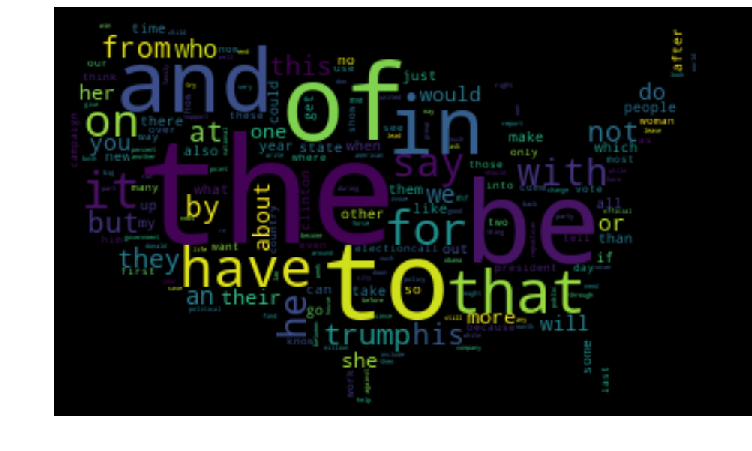
\includegraphics[width=0.8\textwidth]{pictures/real_wordcloud.pdf}
        \caption{Real News}
    \end{subfigure}
    \begin{subfigure}{0.8\textwidth}
        \centering
        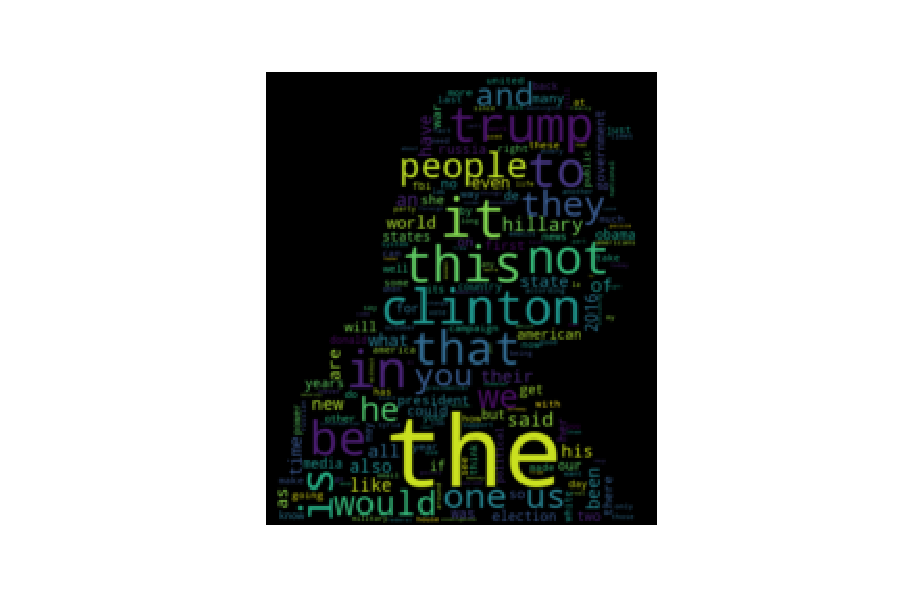
\includegraphics[width=0.8\textwidth]{pictures/fake_wordcloud.pdf}
        \caption{Fake News}
    \end{subfigure}
    \caption{Wordcloud Darstellung des Real News und Fake News 
    Datensatzes. Erstellt mittels der \textsc{wordcloud}-Bibliothek~\cite{wordcloud} }
    \label{fig:WordcloudData}
\end{figure}

Mit dem arithmetischen Mittel der relativen Häufigkeit eines Wortes $\overline{w}$
und dessen Varianz $s$ für die beiden Klassen, lassen sich mit der Diskriminanzfunktion von Fisher 
\begin{equation}
    \label{eqn:fisher}
    S = \frac{(\overline{w_{\text{real}}} - \overline{w_{\text{fake}}})^2}{s_{\text{real}}^2+_{\text{fake}}^2}
\end{equation}
die Wörter finden, an deren Häufigkeiten sich die beiden Klassen gut voneinander trennen
lassen. Anschaulich entspricht dieses dem Verhältnis von Signal zu Untergrund einer Messung und sollte
daher möglichst groß werden. Die Wörter, die sich nach dieser Methode besonders gut zur Klassifizierung
eignen, sind in Abbildung \ref{fig:fisher_hist} dargestellt.

\begin{figure}
    \centering
    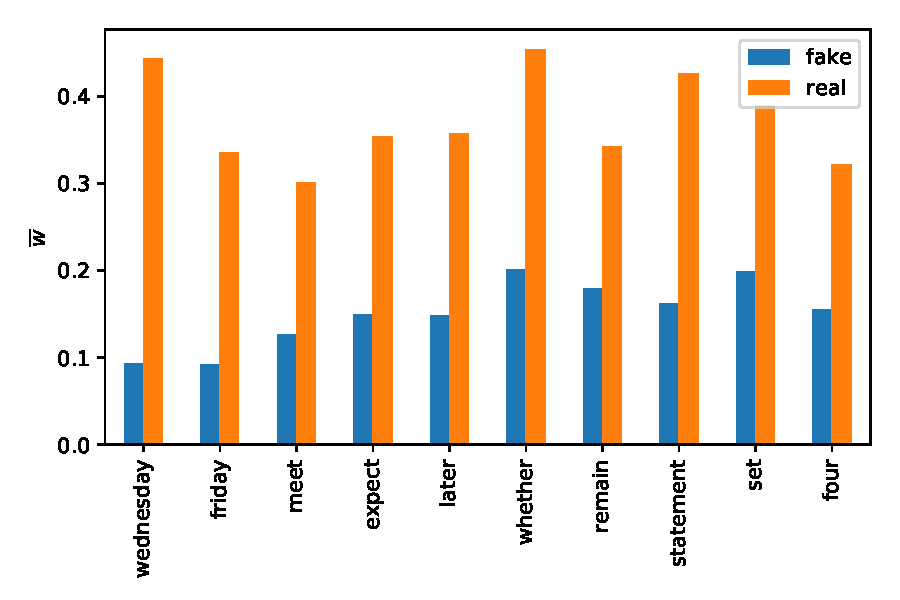
\includegraphics[width=0.8\textwidth]{pictures/data_visualisation.pdf}
    \caption{Hier sind mit der Fisherdiskriminante \eqref{eqn:fisher} bestimmte
    Wörter dargestellt, die sich besonders gut zur Klassifizierung der Texte nach 
    Worthäufigkeiten eignen. Es ist das arithmetische Mittel für die relative Häufigkeit
    eines Wortes in einem Text jeweils für die beiden Klassen dargestellt. }
    \label{fig:fisher_hist}
\end{figure}